\documentclass{article}
\usepackage[utf8]{inputenc}
\usepackage[english]{babel}
\usepackage[font=small,labelfont=bf]{caption}
\usepackage{geometry}
\usepackage{natbib}
\usepackage{pxfonts}
\usepackage{graphicx}
% \usepackage{amsmath}
% \newcommand{\rpm}{\raisebox{.2ex}{$\scriptstyle\pm$}}
% \DeclareMathOperator*{\argmax}{arg\,max}

% \title{Capturing the geometric structure of our experiences and how we remember them}
\title{The fundamental shape of dynamic experiences is preserved in episodic memory}
\author{Andrew C. Heusser \& Jeremy R. Manning}
% \affiliation{Dartmouth College}

\bibliographystyle{apa}

\begin{document}
\maketitle

\section{Abstract}
{
The human memory system is adept at cataloging the rich dynamics of ongoing experience. However, traditional trial-based memory experiments cannot capture these dynamics, and therefore cannot be used to study them.  By constraining participants' experiences in an experiment to occur in temporally discrete trials (and often arranged in a randomized order) the temporal, contextual, and emotional structure of those in-lab experiences necessarily differ from the naturalistic experiences we encounter in everyday life.  Here we investigate how people verbally recall continuous videos by characterizing and relating the thematic dynamics, or ``trajectories,'' of the stimulus and participants' recalls.  Unlike trial-based studies of memory wherein participants attempt to recall the precise stimuli they encounter, naturalistic recall entails capturing the fundamental geometric components of the stimulus topic trajectory.  The precise words participants use to describe the stimulus, and the level of detail and number of distinct events they recall, vary considerably across participants.  Nevertheless, the majority of participants' recall narratives captured the fundamental ``shape'' of the original stimulus.  These findings provide a window into which aspects of naturalistic experiences must be preserved, and which might be more flexible, in considering whether and how those experiences are remembered.

\section{Introduction}

What does it mean to \textit{remember} something? In traditional episodic memory experiments \citep[e.g., list-learning or trial-based experiments;][]{Murd62a, Kaha96}, remembering is often cast as a binary operation: either an item is recalled or it isn't. More nuanced studies might incorporate self-reported confidence measures as a proxy for memory strength, or ask participants to discriminate between ``recollecting'' an experience or a feeling of ``familiarity'' \citep{Yone02}. However, characterizing and evaluating memory in more realistic contexts (e.g., telling a story to a friend about a recent vacation) is a fundamentally different task. Real-world recall is continuous, rather than binary.  The specific words used to describe an experience have very little bearing on whether the experience is considered to have been ``remembered.''  Further, one might remember the gist of an experience but forgot (or neglect to recount) particular details.  Or different people who share an experience might recount the experience with a similar level of detail, but the specific details that were remembered might vary across people.  Which aspects of those recollections should be considered fundamental, and which are extraneous to the main story?

Another major difference between traditional trial-based memory paradigms and real-world memory concerns the subjective experience of the participant.  For example, consider an emotionally salient event in your life (e.g.\ marriage, the birth of a child, death of a loved one, etc.), or even a movie that you were especially impacted by.  No list-learning paradigm (or similar) can hope to capture the nuance and depth of such experiences.  Our everyday experiences feel ``important'' to us, whereas the words we study on a random word list do not.  One component of naturalistic experiences that enhances their impact concerns the temporal structure with which they unfold.  For example, our experiences in the real world are necessarily autocorrelated in space and time on short timescales.  Further, or experiences are often characterized by longer timescale correlations that reflect the impact of our past actions and observations.  These temporal dynamics are not typically present in traditional memory studies, but are important if we wish to understand how our memory systems remember our everyday experiences.

To study the temporal and semantic aspects of memory for naturalistic experiences, we analyzed an open dataset in which participants view and verbally recall an episode of the BBC series \textit{Sherlock}  \citep{ChenEtal17} .  We developed a novel computational approach which combines topic models \citep{BleiEtal03} and hidden Markov models to capture the temporal evolution of rich semantic structure present in naturalistic experiences. We then use this model to characterize the shape and contents of episodic memories for naturalistic experiences. We hypothesized that memory for naturalistic experiences is more about preserving the overall ``shape'' of an experience than any of the particular details.

\subsection{Results}

\begin{figure}[t!]
\centering
\includegraphics[width=1\textwidth]{figs/1_analysis_schematic.pdf}
\caption{\small \textbf{Schematic of the analysis approach.} For each moment of the video, text descriptions were manually generated. Three exemplary time points are displayed here.  Below the video descriptions are text samples from an example participant's verbal recall transcript.  We trained a topic model on the moment-by-moment video description text and transformed participant's recall transcripts using this same model. The bar charts display the resulting topic model weights for the video (in blue) and recall (in orange) for three example topic dimensions.}
\label{fig:schematic}
\end{figure}

\subsubsection{A model to capture the geometric structure of naturalistic stimuli}
We fit a topic model \citep{BleiEtal03} to manually annotated text descriptions of scenes from the episode. The text descriptions contained details of the scene such as the characters, location, and a short summary of the scene (see Fig.\ref{fig:schematic} for example text, see \ref{sec:methods} for analysis details). We then transformed the text descriptions using the (same) topic model, resulting in a scenes (1000) by topics (100) matrix, where each row of the matrix represents a probabalistic mixture of topics discovered in that scene (See Fig.\ref{fig:schematic} for example topic vectors). We expanded this matrix from 1000 to 1976 timepoints by copying the vectors for scenes that spanned multiple TRs. As depicted in Fig.~\ref{fig:model}a, the topics are sparse and change slowly over time. Furthermore, there are clear transitions from one topic `state' to the next, possibly indexing scene transitions in the stimulus.  To get a better handle on this temporal structure, we computed the timepoint-by-timepoint correlation matrix of the video model (Fig.~\ref{fig:model}b).  This correlation matrix reveals that the model has a strong, block-diagonal structure. Another interesting feature is that there is very little correlation between blocks (i.e. the off-diagonal values are small). This is an interesting feature of the model because to the extend that the blocks represent `events' in the video, the model representations of those events are unique and highly discriminable.

\subsubsection{Modelling verbal free recall}
After watching the episode, participants verbally recalled (in order) as much as they could.  We used the same topic model (fit with the text descriptions of the video) to transform participants' verbal recall transcripts. The result was a sentences (range: X to X) by topics (100) matrix for each participant, where each row represented the estimated mixture of topics for a given window of sentences during recall. In order to average the recall models across participants, we resampled each model at the resolution of the video model (1976 timepoints). The individual models can be seen in Supp Fig X and the group average is plotted in Fig.~\ref{fig:model}c. Note that the topics were derived solely from the text descriptions of the video, and so the topic models estimated for recall are dependent on the topics in the episode. In effect, this approach projects the participants' verbal recall into the video 'stimulus space', allowing us to quantify the dynamics of verbally reported memories as well as relate them to their originating experiences.

Next, we investigated the temporal structure of the recall matrices. For each participant, we computed a timepoint-by-timepoint correlation matrix from recall models. Like the video model, each participant's recall correlation matrix exhibited a block-diagonal structure (Supp Fig X). To visualize the group average, we resampled all of the recall models to the duration of the video model (1976 timepoints), computed the timepoint-by-timepoint correlation matrices and then averaged across participants.  The average recall matrix also had a block-diagonal structure, albeit smoother than the video model (Fig.~\ref{fig:model}d).

\subsubsection{Bridging between the stimulus and recall}
The participants in this study were instructed to recall as much of the episode as they could in the order it happened.  Thus, we hypothesized that the recall models should resemble the video model to the extent that participants followed these instructions and had reasonably good memory accuracy. To test whether this was true, we correlated each moment of the video model with each moment of each participants' resampled recall model. We then averaged these matrices together to get a single group averaged matrix.  The result was a viewing time (1976) by recall time (1976) correlation matrix representing the average relationship between every moment of the movie and recall models (Fig.~\ref{fig:model}e). Notably, we observe significant correlation values (p<.05, permutation test described in \ref{sec:methods}) primarily along the diagonal, suggesting that our model captures the fact that participants recalled the episode in order. We also visualized this effect by projecting the matrices into a 3D space (reduced using Spectral Embedding [cite]) where the proximity of the trajectories at every timepoint represents how similar the topic vectors were. Visualizing the data in this way makes it clear that the overall shape and correlational structure of the video and average recall matrices is quite similar.

\begin{figure}[ht!]
\centering
\includegraphics[width=\textwidth]{figs/2_eventseg_v4.pdf}
\caption{\small \textbf{Modelling naturalistic stimuli and recall.} For all plots, darker colors indicate greater values and the range of each plot is 0-1.  A). A timepoints (1976) by topics (100) matrix representing the video stimulus.  Each row represents the most likely mixture of topics for a given timepoint. Each columns represents a different topic. B). A timepoints (1976) by topics (100) matrix representing participant \#13's recall. C). A viewing-time (1976) by viewing-time (1976) correlation matrix representing the correlation of each moment of the video model with every other moment of the video model. The white boxes represent `events' recovered by a hidden Markov model. D). A recall-time (294 sentences) by recall-time (294) correlation matrix for participant \#13. E). An events (34) by topics (100) matrix where each row represents the average topic vector for each event in the video model.  F). An events (27) by topics (100) matrix where each row represents the average topic vector for each event in participant \#13's recall model. G. A recall events (27) by video events (34) correlation matrix for participant \#13. The yellow squares identify the video event with the highest correlation to a given recall event. F. A group averaged recall events (34) by video events (34) correlation matrix.  The yellow squares identify the video event with the highest correlation to a given average recall event.}
\label{fig:model}
\end{figure}

\subsubsection{Segmenting the video and recall models into `events'}
One prominent feature of the video and recall correlation matrices (see Fig.~\ref{fig:model}) is a strong, block structure along the diagonal of the matrices.  We hypothesized that this structure might arise from transient stability in the language used to describe each event of the video. If true, we reasoned that it would be possible to decode which particular event a participant is describing by comparing the average topic model for a particular recall `event' with the average topic vector for each video event. Following this logic, the video event that is most similar to the given recall event would be the event the participant is most likely describing.  To test this idea, it is first necessary to systematically parse the matrices into events.  To do this, we leveraged a hidden Markov model (~\citep{BaldEtal17}) to estimate $k$ events from a (multivariate) time series. The algorithm determined 34 events for the movie model and a range of values (range=8-27, mean= 15.41, SD=5.6) for the recall models (see ~\ref{sec:methods} for details on choosing $k$).  The events discovered for a representative participant are highlighted in \ref{fig:model}b.

Next, we hypothesized that the individual `blocks' along the diagonals of the recall matrices represent the recall of a particular video event. To test this, first we created a video event model, which was done by averaging together neighboring topic vectors that the were classified to be in the same event (Fig.~\ref{fig:model}c), resulting in an events (34) by topics (100) matrix.  We performed the same procedure for the recall matrices (see Fig.~\ref{fig:model}d for example). Then, we computed the correlation between these two event models, resulting in a video events (34) by recall events (8-27, depending on the participant) correlation matrix (see Fig/~\ref{fig:model}e). These matrices represent the extent to which each recall event is similar to each video event (for each participant). To determine which video events the recall events most likely referred to, for each recall event, we found the index of the video event with the highest correlation (i.e. the argmax).  This is depicted in Fig.~\ref{fig:model}e as the cell highlighted with the black box for each column in the video-recall event correlation matrix. Notably, our algorithm suggests that the example participant recalled the events largely in order (occasionally skipping over an event).

Next, we computed a group-averaged recall event model and video-recall event correlation matrix (Fig.~\ref{fig:model}f).  To do this, for each participant (and each recall event), we grouped the recall event vectors (across all participants) by the video event that they were most highly correlated to. We then averaged the recall event vectors within group. This yielded an average recall event vector for all but one (of 34) event (since no participant remembered this event according to our model). Lastly, we computed an average recall event (34) by video event (34) correlation matrix, and highlighted the highest correlation in the column with a black box (Fig.~\ref{fig:model}f). Notably, this matrix displayed high correlation values along the diagonal and low correlations in the off-diagonal cells. This suggests that on average, participants were able to recapitulate the events in the episode and our model was sensitive enough to capture this behavior.
% NOTE: ^ Need a null model for the group analysis.  I think it could be to get a result that looks like this even if we scrambled the text. My concern is that I'm grouping the recall events by the video event they were most similar to, and then averaging, which may give rise to a smooth looking plot without any real information there...

\begin{figure}[t!]
\centering
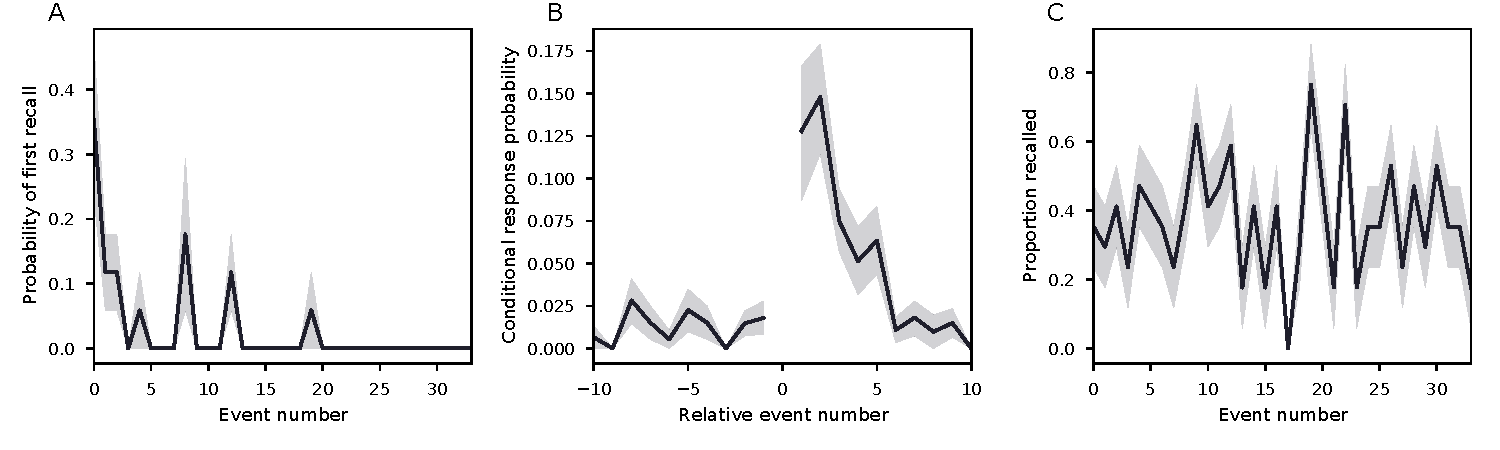
\includegraphics[width=1\textwidth]{figs/3_list_learning.pdf}
\caption{\small \textbf{Naturalistic extensions of classic memory analyses.} A). The probability of first recall as a function of the serial position of the event during encoding. B). Given recall of event i, the probability that the next recalled item will be from serial position i +/- lag. C). Proportion recalled as a function of serial position. All error bars are the standard error of the mean derived from a bootstrap resampling procedure.}
\label{fig:list-learning}
\end{figure}

\subsubsection{Naturalistic extensions of classic memory analyses}
Just like in a traditional `free-recall' list-learning experiment where participants view a list of words and then verbally recall them, our video-recall matching approach described above affords us the ability to analyze memory in the same way (where the recalled words are analogous to recalled events). In our first set of analyses, we sought to characterize memory performance/dynamics by extending classic analyses originally designed for list-learning experiments to more naturalistic settings.

First, we asked whether the estimated number of recall events ($k$) by participant was related to hand-annotated accuracy as published in Chen et al. (2017).  We found a strong positive correlation where subjects with a greater number of recall events also had better memory performance (Pearson's $r$(16)=.67, $p$=.003). Thus, the block-diagonal temporal structure in the recall matrices computed by our model is strongly related to the variability in memory performance across participants.  We considered two additional across-participant measures of recall that characterize memory organization: temporal clustering and semantic clustering. Temporal clustering (as described in REF) measures the extent to which participants tend to cluster recalls of events encoded nearby in time.  For example, if a participant recalled in exact serial order, the score would be 1 whereas if they sequentially recalled randomly positioned items the score would be ~.5.  We found that participants who clustered in time also recalled a greater number of events (Pearson's $r$(16)=.62, $p$=.007). Next, we assessed semantic clustering.  Similar to temporal clustering, semantic clustering measures the extent to which participants cluster their responses by semantic similarity.  We used the topic vector representations of each event as a proxy for semantic information contained in that event.  For each transition, we computed the rank percentile of the of the correlation between the the current event and then next event. For example, if a participant sequentially recalled events where each successive recall was the event that was most semantically similar to the previous, the semantic clustering score would be 1.  If the events were recalled in a random order with respect to semantic information, the clustering score would be ~.5. We found that the semantic clustering score was related to memory performance across participants (Pearson's $r$(16)=.55, $p$=.02).  Thus, participants who organized their recalls with respect to the semantic information contained in the scene had better memory performance.

Then, we considered initiating the recall sequence (known in the literature as the `probability of first recall' or `PFR'). This metric quantifies the likelihood of initiating a sequence of recalls based on the item's serial position. We found that participants tended to initiate their recall sequences with the first few events (Fig.~\ref{fig:list-learning}a), which is qualitatively very similar to previously published list learning experiments (REF).  Next, we considered another well-studied memory measure in list-learning, the lag conditional response probability curve (or lag-CRP). Given the recall of a stimulus in study position $n$, the lag-CRP quantifies the probability that the next item recalled will be of lag $i$. The results suggest a strong bias to transition sequentially in the forward direction Fig.~\ref{fig:list-learning}b. This can be seen by the high probability values in the lag ~1-5 positions compared to the rest of the transition possibilties. Notably, participants were instructed to recall as much as they could in order, and the shape of this lag-CRP is qualitatively similar to list-learning studies of serial recall (REF), where participants are required to recall lists of words in their serial order. Finally, we assessed memory performance for each event in the video. This plot quantifies the proportion of participants that recalled each event in the video (Fig.~\ref{fig:list-learning}c). We found that there was substantial variability in memory for the different events. % NOTE: whats the right stat for this?

\subsubsection{The fundamental shape of an experience is preserved in recall}
The previous set of analyses are useful in that they enable us to quantify memory dynamics for naturalistic stimuli in a way that is comparable to a vast literature on list-learning recall dynamics. However, these methods fail to capture the rich semantic and temporal structure present in naturalistic stimuli (and associated recall of those experiences). Thus, our next set of analyses test whether the `shape' of an experience is preserved in memory. We hypothesized that despite individual variability in the precision and amount of content recalled across subjects, the general shape of the episode would be recalled by everyone.

\begin{figure}[t!]
\centering
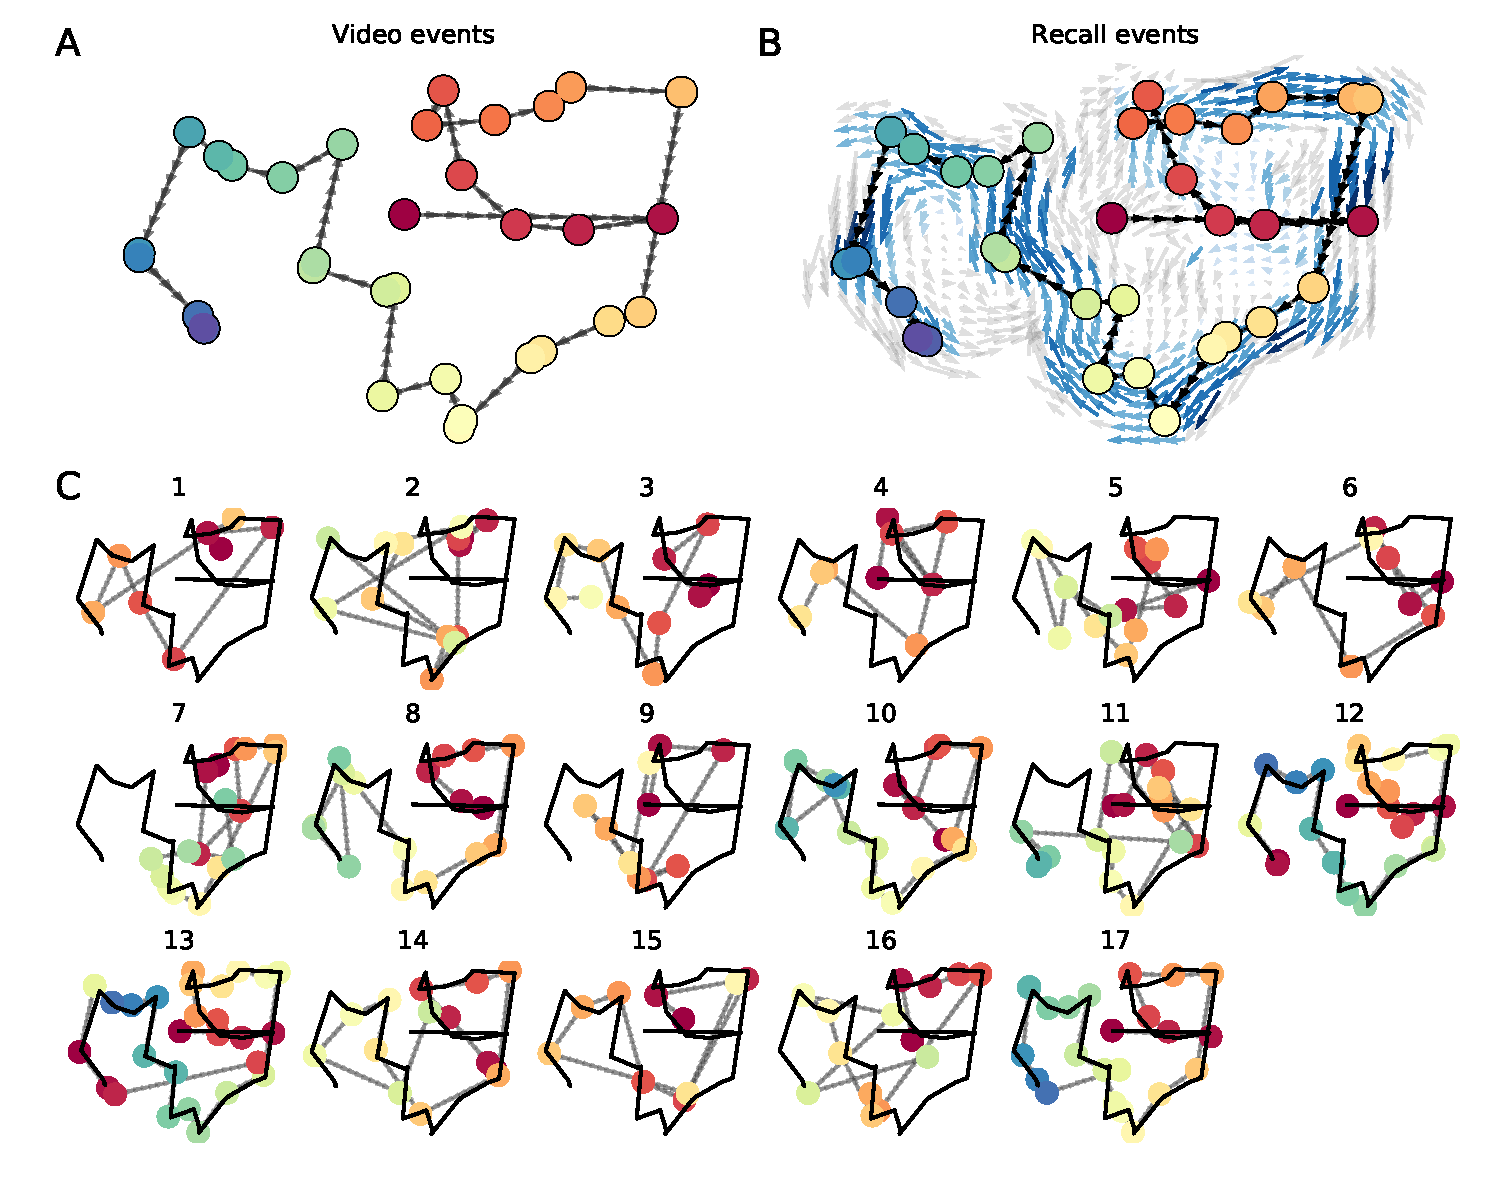
\includegraphics[width=1\textwidth]{figs/4_trajectory.pdf}
\caption{\small \textbf{Video and recall trajectory plots.} A). 2-dimensional embedding of recall events model. The arrows indicate the forward direction of the video events. B). 2-dimensional embedding of the average recall events.  The colors refer to the most similar video events.  The lines connecting the points represent the average probability of transitioning from one event to the other. The weight of the line is proportional to the transition probability.}
\label{fig:trajectory}
\end{figure}

To better visualize the relationship between the video and recall event models, we embedded the video and average recall model into a 2D space (using the UMAP dimensionality reduction algorithm, for details see \ref{sec:methods}) where the points represent video/recall events and the distance between them represents their similarity in 'topic space' (Fig.~\ref{fig:trajectory}a). (Note that all analyses are performed in the original 100 dimensional space.) We computed the group average transition probabilities from each event to each other event and plotted the values as lines where the tranparency is proportional to the probability of the transition (Fig.~\ref{fig:trajectory}b).  Visual inspection reveals that the two models have a very similar geometric structure, and the transition probabilities tend to be strongest between events that occured sequentially (or nearby) in time.

% To explore individual variability (and consistency) in the recall event models, we embedded each participant's recall event model in the same 2D 'topics space' described above (\ref{fig:model}h). Despite the variability in the number of events remembered, the overall shape of most of the participants' recall trajectories are similar to the video model (\ref{fig:model}h), particularly the participants with a greater number of recalled events.

To formalize the observation that participants' recall trajectories generally matched the shape of the video trajectory, we fit participants' recall data to a model comprised of $k$ line segments that were connected by the average recall event coordinates. We fixed the endpoints of the model at the average first and last recall event, but fit the placement/length of rest of the segments to the data using the average recall events as `hinge-points'. Using a cross-validated model fitting procedure (see ~\ref{sec:methods} for details), we searched for the optimal number of line segments. The best fitting model ($k$=11) can be seen in Fig.~\ref{fig:linesegs}. This model represents the set of consecutive line segments that best describe participant's recall trajectories. Notably, the optimal model comprises a subset of the total recall events (~roughly 1/3).

We hypothesized that the `hinge-points' between line segments represent critical scenes of the video where the storyline changed direction. To get a sense of the semantic content of each hinge-point, we created wordles (left side of each wordle) where the size of the word is proportional to its frequency in the video text descriptions for that event (Fig.~\ref{fig:linesegs}). We performed the same analysis for the recall text (right side of each wordle).  Notably, the text in the worldes is distinct across hinge-points, but but similar between video and recall within hinge-point.

% NOTE: WILL ADD ANOTHER PARAGRAPH HERE IF THE 'TOPIC FLOW' ANALYSES WORK OUT

\subsubsection{Measuring the quality of recall}
Representing the video and verbal recall as events in `topic space' also affords us the ability to characterize the quality of recall in a more fine-grained and nuanced way than what was previously possible. To quantify the similarity between the video model and individual recall models, we considered a number of novel metrics.  First, we tested whether each participant's recall model matched the movie model in a general sense. To do this, for each participant we filtered the video model to only include the events that the participant remembered. Then, we computed the root mean squared difference (RMSD) between the video model and the recall model. As an example, if the participant remembered all the events in order (with perfect precision), the expected distance value would be 0. However, if they remembered a subset of events, events our of order or with low precision the expected distance would be greater than 0. To assess significance, we performed a permutation test where we circularly shifted the recall model (10000 times) and recomputed the RMSD. The recall model significantly matched the video model for nine of the participants [p<.05; participants: 3-4, 8-13, 17 and the p-value for the rest of the participants was less than .25]. Furthermore, the RMSD values were significantly correlated to memory performance across participants [Pearson's r(16)=-.57, p=.016]. Thus, a closer match between the video and recall event models was related to better recall performance.

Next, we tested whether participants who recalled more events were also more precise in their recollections. For each participant, we computed the correlation between each recall event and its matching video event (only for the events which they recalled). This resulted in a single number for each recalled event indexing how similar the recall event was to its matching movie event (i.e the `precision' of the recall). We then averaged the correlations within participant. In line with our prediction, there was a strong correlation between memory performance and precision suggesting that participants who remembered more events also remembered them more veridically [Pearson's r(16)=.74, p=.0006]. Next, we considered the distinctiveness of each recall event. That is, how uniquely a recall event matched a given video event compared to all other video events. We hypothesized that participants with high memory performance might describe each event in a more distinctive way (relative to those with lower memory performance who might describe events in a more general way). To this end, we computed a `distinctiveness' score for each participant (i.e. 1 - the correlation between a recall event and all non-matching video events).  Then, we averaged this measure over recall events within participant.  We found that participants with higher memory performance also had higher distinctiveness scores [Pearson's r(16)=.8, p=.0001].

Lastly, we tested whether participants with better memory performance were also more likely to remember the events in order.  For each participant, we computed the Spearman rank correlation between the order of events that the participant recalled and the actual order of events (filtering events that were actually recalled).  We found that participants who recalled more events also recalled more of them in order [Pearson's r(16)=.5, p=.04]. In summary, we found that better memory performance was associated with more precise and distinctive recall.

\bibliography{memlab}
\end{document}
